\chapter{Related Work}
\label{c:related_work}

In this chapter we discuss two types of related work. The first consists of existing OWASP MASTG reference apps for Android. The second is about academic publications that rely on the MASTG.

% Struktur
\section{State-Of-The-Art in OWASP MASTG Reference Apps}
There are 19 MASTG reference apps listed on the OWASP page \citep{owasp_reference_app_website} and its corresponding GitHub repository \citep{mastg_repo_apps_overview} at the time of writing. To evaluate the state of the art of MASTG reference apps, we examine each one of them in order to identify and categorize their implemented vulnerabilities. Only eight of these apps have both available source code and some form of documentation of their vulnerabilities. The vulnerabilities were then mapped to their corresponding OWASP Mobile Application Security Weakness Enumeration (MASWE) counterparts, which lists and discusses the vulnerabilities that the MASTG tests for.

\subsection{Methodology}
We evaluated 19 MASTG reference apps as to whether their source code is available online, and if so, whether they have any documentation of their weaknesses. The app selection includes four "Android Uncrackable" reference apps, named L1 \citep{android_uncrackable_l1}, L2 \citep{android_uncrackable_l2}, L3 \citep{android_uncrackable_l3} and L4 \citep{android_uncrackable_l4}. None of them have any documentation on their implemented weaknesses and are excluded from this review because of it. The other apps excluded for the same reason are: Android License Validator \citep{license_validator}, DVHMA \citep{dvhma}, Digitalbank \citep{digitalbank}, DodoVulnerableBank \citep{dodo_vulnerable_bank}, disable-flutter-tls-verification \citep{disable_flutter_verification_app}, and MASTestApp-Android-NETWORK \citep{mast_test_app_android_network}. The MASTG-Hacking-Playground-Kotlin-App \citep{mastg_hacking_playground_kotlin} has been excluded from this literature review because we have included and evaluated an identical Java version of this app. 

The following apps have been included in the review: AndroGoat \citep{andro_goat}, DIVA Android \citep{diva_android},  InsecureBankv2 \citep{insecure_bank_v2}, MASTG-Hacking-Playground \citep{mastg_hacking_playground}, OVAA \citep{ovaa}, InsecureShop \citep{insecure_shop}, Finstergram \citep{finstergram}, and Android BugBazaar \citep{android_bugbazaar}. A summary of this selection process can be seen in Table \ref{overview_reference_apps_sourcecode_and_documentation}.

\begin{table}[htpb]
\centering
\caption{Overview of the availability of source code and documentation of MASTG reference apps, and whether they were included in our analysis}
\label{overview_reference_apps_sourcecode_and_documentation}
\begin{tabular}{ |p{3cm}||p{3cm}|p{3cm}|p{3cm}|  }
    \hline
    \multicolumn{4}{|c|}{OWASP MASTG Reference Apps} \\
    \hline
    App name& Source code & Documentation & Included \\
    \hline
    Uncrackable L1   &  &  &  \\
    \hline
    Uncrackable L2   &  &  &   \\
    \hline
    Uncrackable L3   &  &  &   \\
    \hline
    Uncrackable L4   &  &  &   \\
    \hline
    License Validator   &  &  &   \\
    \hline
    DVHMA   &  &  &  \\
    \hline
    Digitalbank   & \centering\checkmark &  &    \\
    \hline
    Dodo Vulnerable Bank   & \centering\checkmark &  &  \\
    \hline
    disable-flutter-tls-verification   & \centering\checkmark &  &  \\
    \hline
    MASTestApp-Android-NETWORK   & \centering\checkmark &  &  \\
    \hline
    MASTG-Hacking-Playground-Kotlin-App  & \centering\checkmark & \centering\checkmark &  \\
    \hline
    AndroGoat  & \centering\checkmark & \centering\checkmark & \centering\arraybackslash\checkmark \\
    \hline
    DIVA Android  & \centering\checkmark & \centering\checkmark & \centering\arraybackslash\checkmark \\
    \hline
    InsecureBankv2 & \centering\checkmark & \centering\checkmark & \centering\arraybackslash\checkmark \\
    \hline
    MASTG-Hacking-Playground & \centering\checkmark & \centering\checkmark & \centering\arraybackslash\checkmark \\
    \hline
    OVAA & \centering\checkmark & \centering\checkmark & \centering\arraybackslash\checkmark \\
    \hline
    InsecureShop & \centering\checkmark & \centering\checkmark & \centering\arraybackslash\checkmark \\
    \hline
    Finstergram & \centering\checkmark & \centering\checkmark & \centering\arraybackslash\checkmark \\
    \hline
    BugBazaar & \centering\checkmark & \centering\checkmark & \centering\arraybackslash\checkmark \\
    \hline
\end{tabular}
\end{table}

\subsection{Findings}
Across the eight evaluated OWASP MASTG reference apps, 163 weaknesses were implemented. We mapped them to their respective MASWE counterparts and grouped them by their vulnerability category (Storage, Crypto, Auth, etc.). An overview of the apps and their implemented vulnerabilities can be seen in Table \ref{overview_reference_apps_vulnerabilities_per_category_each}.

\begin{table}[htpb]
\centering
\small
\caption{Mapping of MASTG reference apps vulnerabilities to their MASVS categories}
\label{overview_reference_apps_vulnerabilities_per_category_each}
\begin{tabular}{ |p{1.75cm}||p{1.3cm}|p{0.9cm}|p{0.9cm}|p{0.9cm}|p{0.9cm}|p{0.9cm}|p{0.9cm}|p{0.9cm}|p{0.9cm}|  }
    \hline
    \multicolumn{10}{|c|}{OWASP MASTG Reference Apps} \\
    \hline
    App name & \# Vuln. & Stora. & Crypt.  & Auth  & Netwo.  & Platf.  & Code  & Resil.  & Priva. \\
    \hline
    AndroGoat & \centering24 & \centering7 & \centering1 & \centering1 & \centering4 & \centering8 & \centering1 & \centering2 &  \\
    \hline
    DIVA & \centering13 & \centering5 &  & \centering5 &  &  & \centering3 &  &  \\
    \hline
    InsecureB. & \centering25 & \centering4 & \centering2 & \centering4 & \centering1 & \centering8 & \centering1 & \centering5 &  \\
    \hline
    Playground & \centering15 & \centering5 & \centering1 &  & \centering1 & \centering3 & \centering3 & \centering2 &  \\
    \hline
    OVAA & \centering18 & \centering1 & \centering1 &  &  & \centering10 & \centering6 &  &  \\
    \hline
    Ins.Shop & \centering19 & \centering2 &  & \centering2 & \centering1 & \centering13 &  & \centering1 &  \\
    \hline
    Finster. & \centering5 &  &  &  &  & \centering3 & \centering2 &  &  \\
    \hline
    BugBaza. & \centering44 & \centering7 &  & \centering1 &  & \centering23 & \centering10 & \centering3 &  \\
    \hline
\end{tabular}
\end{table}


\subsubsection{Lack of vulnerability documentation}
A recurring issue with many of the reference apps lies in their documentation of the implemented vulnerabilities. 11 of the reference apps listed by the OWASP MASTG do not have any documentation of their weaknesses at all, which led to their exclusion from this evaluation. The apps that do include some form of documentation of their vulnerabilities do so in a very minimal way. Most often, the documentation consists of a single list that merely names the implemented weaknesses. None of the apps map the implemented weaknesses to their OWASP MASWE counterparts. Only two apps \cite{finstergram, mastg_hacking_playground} actually document what the weaknesses entail, how they are implemented, and how to fix or exploit them. 

This additional documentation is not necessary for the apps to function as a penetration testing practice environment. But lacking it does reduce their value as an educational resource in reference to the MASTG. A simple mapping of the implemented vulnerabilities to their respective MASWE counterparts helps mobile developers better connect the theoretical concepts provided by the MAS project with the practical environment of the reference apps. By providing no documentation on the implemented weaknesses, developers using the apps to learn are unable to verify which vulnerabilities they have found and which ones they have not. This hinders them in assessing their skills in detecting and exploiting mobile security vulnerabilities, which negatively impacts the educational value provided by the apps. The apps adequacy and function as a mobile security tool testing benchmark are much affected in the same way. If there is no documentation of the vulnerabilities implemented, it becomes extremely difficult to reliably assert how many of the vulnerabilities found by the tools are part of the intentionally created set and how many of the intentionally implemented ones have been missed by the tools. This means that without any documentation of the implemented vulnerabilities, the MASTG reference apps are just as unfit for benchmarking SAST and DAST tools as any real-world apps dataset. The apps we develop aim to address this issue by documenting all implemented weaknesses, including a mapping of the implemented vulnerabilities to their respective MASWE counterparts. Additionally, each implemented vulnerability will contain documentation on where it is found, which lines of code are relevant, how it can be exploited, and sometimes how it can be fixed.

\subsubsection{Uneven distribution of vulnerability coverage}
At the time of writing, there are a total of 117 MASWE vulnerabilities across eight categories documented by OWASP \cite{owasp_maswe_website}. Of these 117 vulnerabilities, only 42 are actually covered by any of these reference apps. 

The eight apps together have 163 implemented weaknesses that can be mapped to only 42 different types of vulnerabilities as defined by MASWE. Because there are 117 different vulnerability types, this leaves a total of 75 vulnerabilities, as documented and classified by OWASP MASWE and referenced in the MASTG, completely without representation. This means that the vulnerabilities implemented in the MASTG apps serve as a reference to only a minority of the MASWE vulnerabilities. While the vulnerability types that make up this minority are covered on average almost four times, the vast majority of vulnerability types goes completely without a practical reference in the MASTG apps. 

To make this point more clear; the ten most frequently covered vulnerabilities are implemented a total of 87 times, as seen in Figure \ref{fig:ten_most_frequently_covered_maswe_vulnerability_types}. This means that they represent 53.4\% (87/163) of all implemented vulnerabilities, despite only covering 8.5\% (10/117) of all vulnerability types as referenced by MASTG. The most frequently implemented vulnerability is MASWE-0066, which deals with insecure intents. Of the ten most frequently covered vulnerabilities, five are of the category MASVS-Platform.

\begin{figure}[htbp]
  \centering
  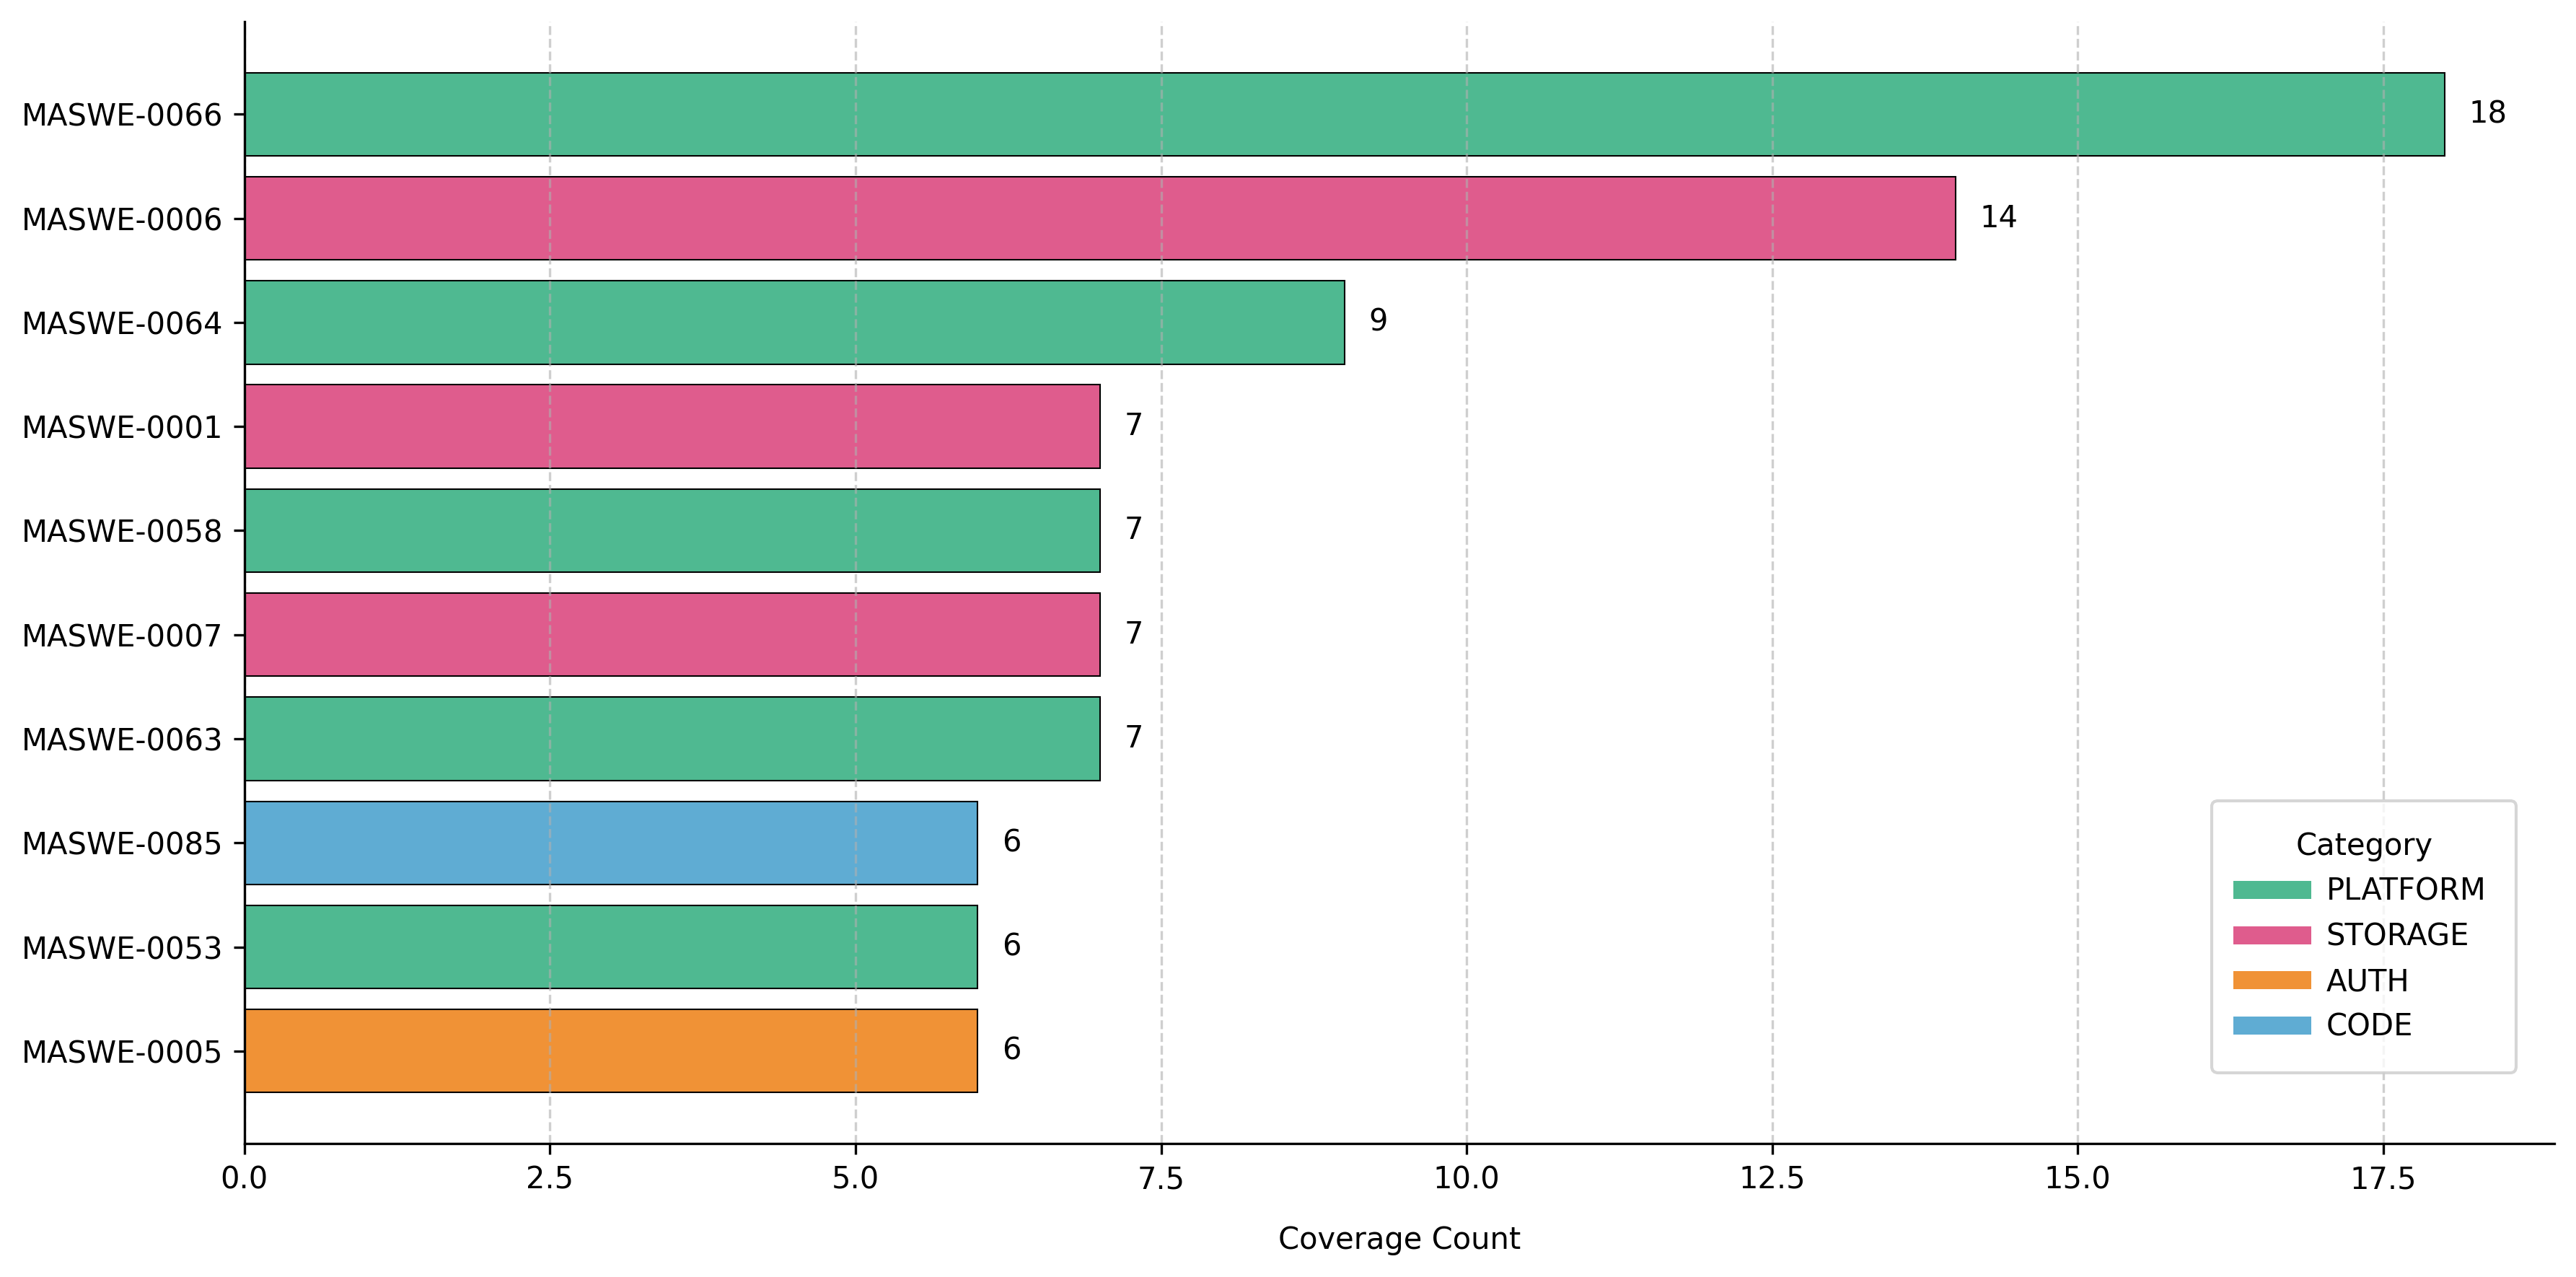
\includegraphics[width=1.0\textwidth]{figures/related_work/top_10_vulnerabilities.png}
  \caption{Ten most frequently covered types of OWASP MASWE vulnerabilities}
  \label{fig:ten_most_frequently_covered_maswe_vulnerability_types}
\end{figure}

\subsubsection{Coverage of vulnerability categories}
There is not only a favoring of certain specific MASWE vulnerabilities, but an uneven coverage of the vulnerability categories themselves as well. The percentage-wise coverage of MASVS categories can be seen in Figure \ref{fig:vulnerability_coverage_percentage_without_own_apps}. Some categories see a high percentage of their vulnerabilities covered, such as MASVS-PLATFORM with 72.7\% or MASVS-STORAGE with 66.7\%. Others see very little to no coverage at all, such as MASVS-CRYPTO with 21.1\% and MASVS-AUTH with only 10\%. Worst of all is MASVS-PRIVACY, with a vulnerability coverage of 0\%.

\begin{figure}[htbp]
  \centering
  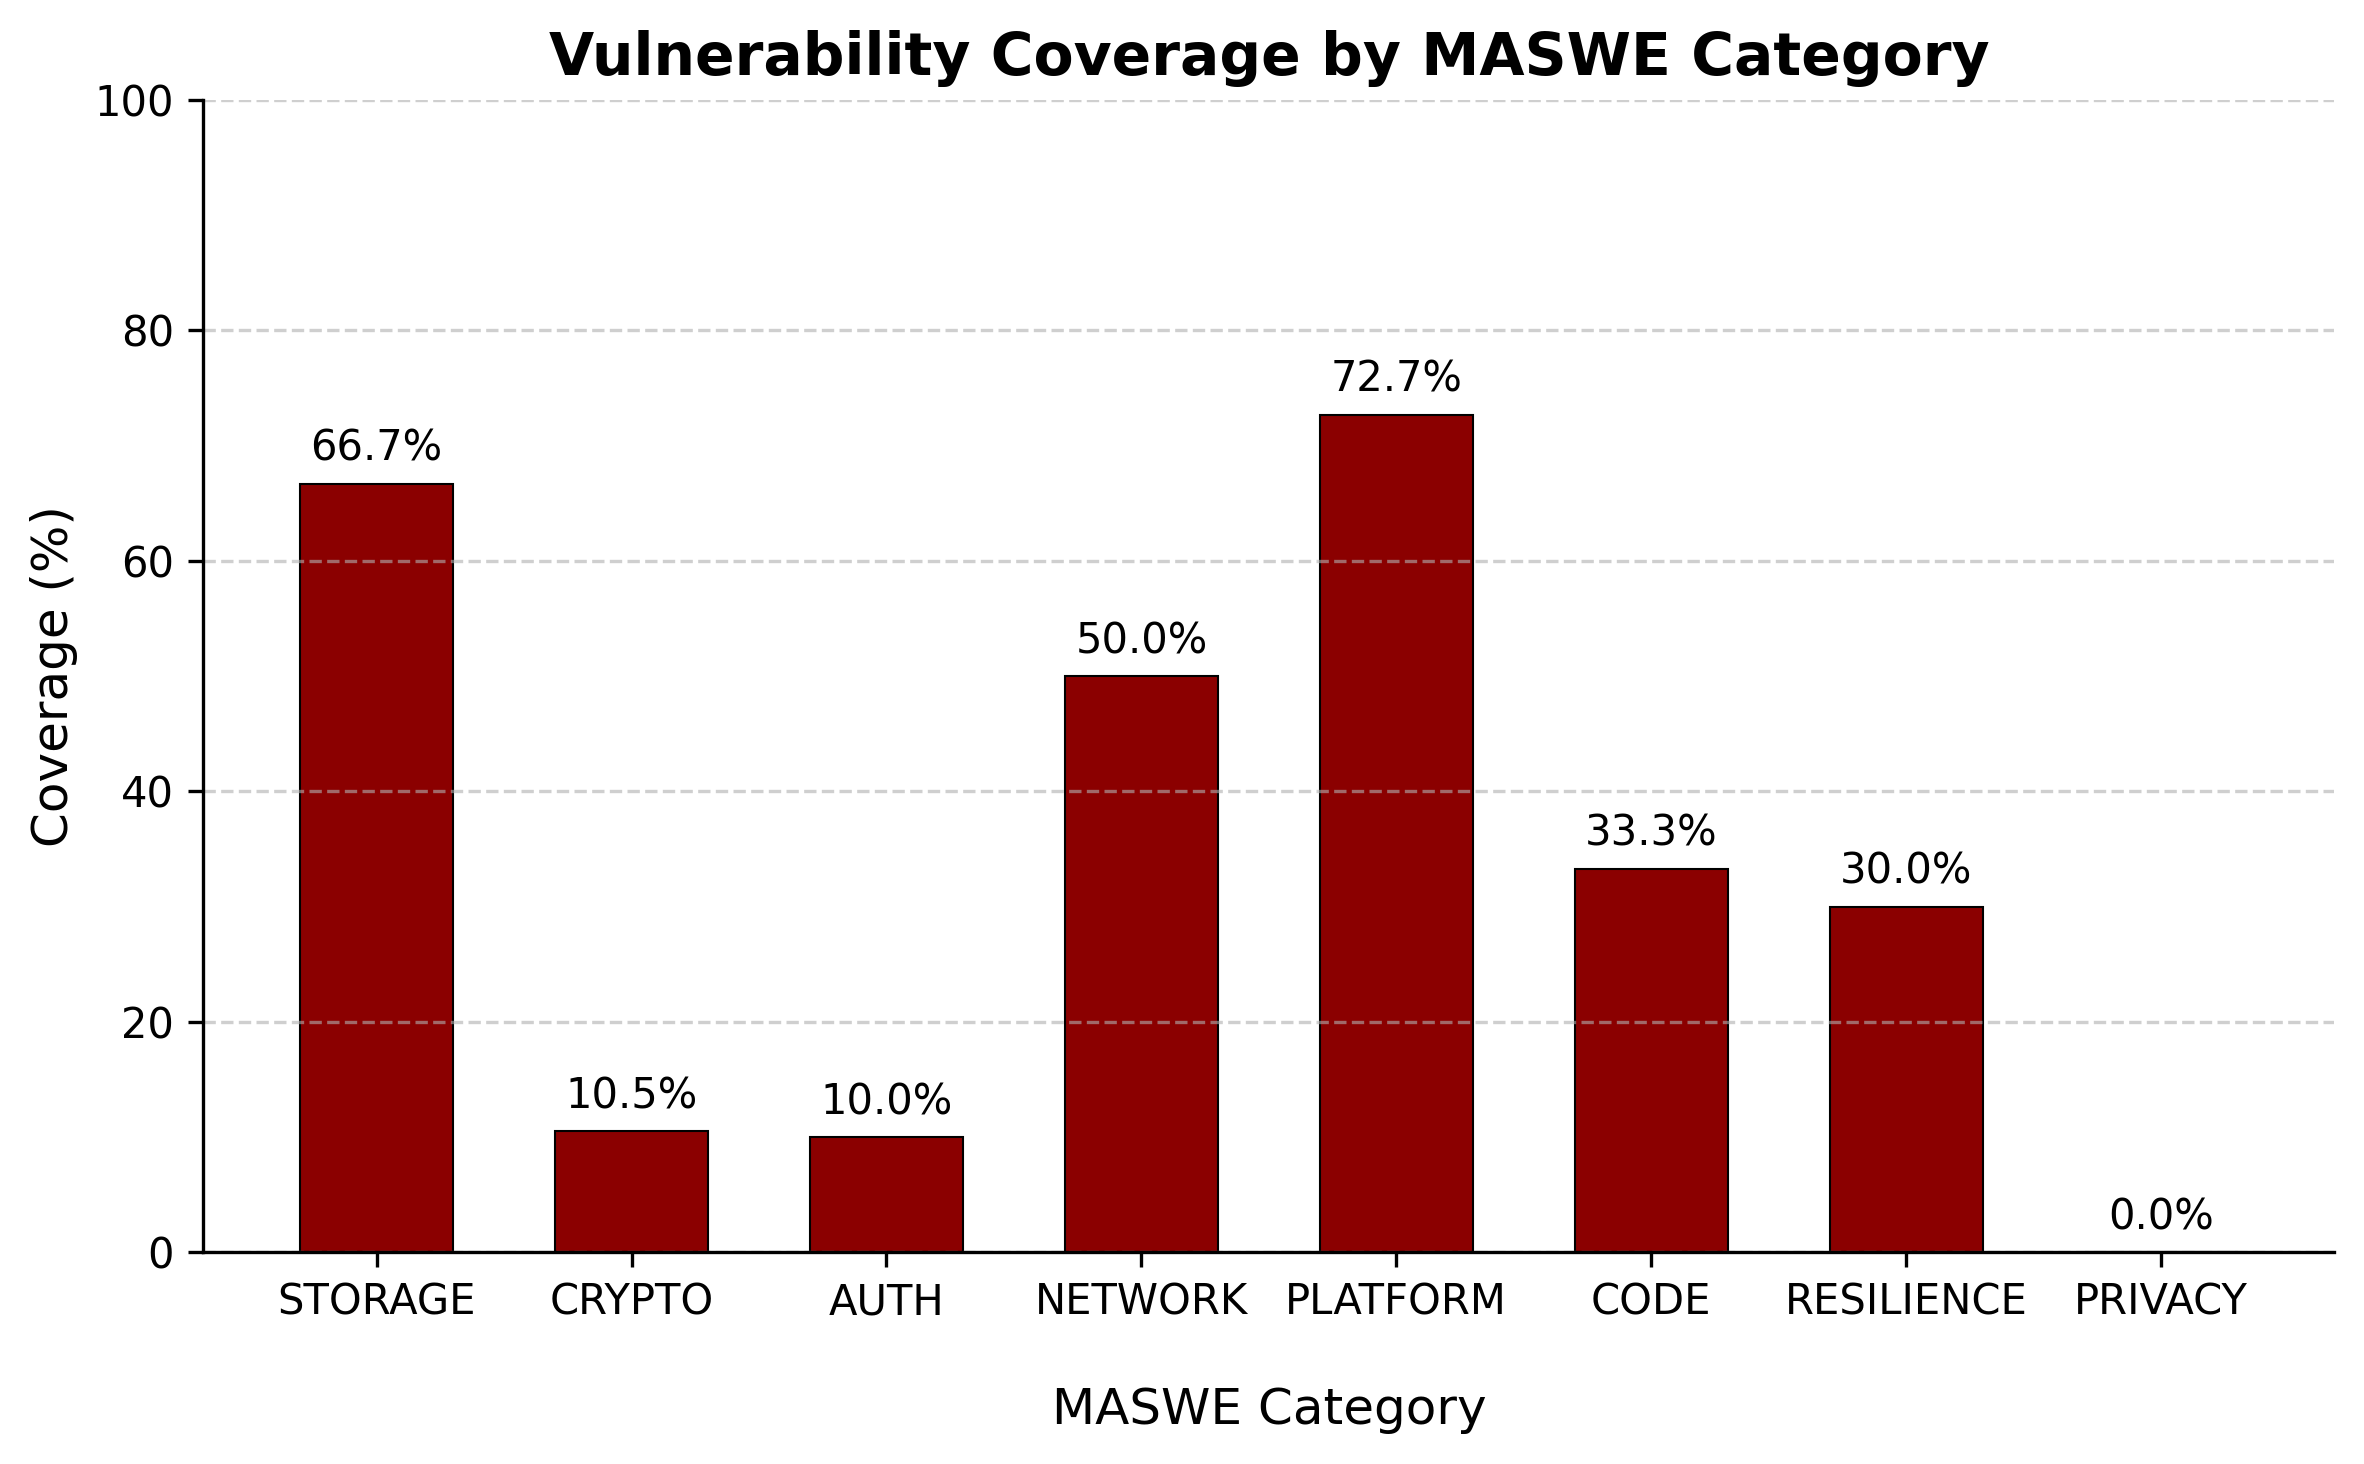
\includegraphics[width=1.0\textwidth]{figures/related_work/vulnerability_coverage_percentage.png}
  \caption{Relative coverage of MASVS categories}
  \label{fig:vulnerability_coverage_percentage_without_own_apps}
\end{figure}

Viewing the coverage in absolute rather than percentage values makes it look slightly more even. As seen in Figure \ref{fig:vulnerability_coverage_absolute_without_own_apps}, all but two categories have between two and seven of their types of vulnerabilities covered. The only outliers are the categories MASVS-PLATFORM, which has a total of 16 out of 22 vulnerabilities implemented, and MASVS-PRIVACY, which has no vulnerabilities covered at all. This shows that vulnerabilities are covered rather evenly across the 8 categories, regardless of the number of vulnerabilities each category has to offer, which explains the large differences in percentage-wise coverage seen in the previous Figure \ref{fig:vulnerability_coverage_percentage_without_own_apps}. This does not mean that the coverage of the different MASVS categories is proportional, as larger categories should have a larger group of vulnerabilities implemented than smaller ones when viewed in absolute numbers. This further reinforces the fact that the vulnerability categories are not covered evenly.

The remarkably high coverage of MASVS-PLATFORM vulnerabilities coincides with the findings shown in Figure \ref{fig:vulnerability_coverage_percentage_without_own_apps}; not only are 5 of the 10 most frequently covered vulnerability types part of MASVS-PLATFORM, but the category itself is also the most broadly implemented category when compared to the others. The complete lack of coverage of MASVS-Privacy vulnerabilities can in part be accounted for by the fact that the category itself is newer than the other seven, having been introduced in MASVS version 2.1.0 \cite{owasp_introducing_masvs_privacy}.


\begin{figure}[htbp]
  \centering
  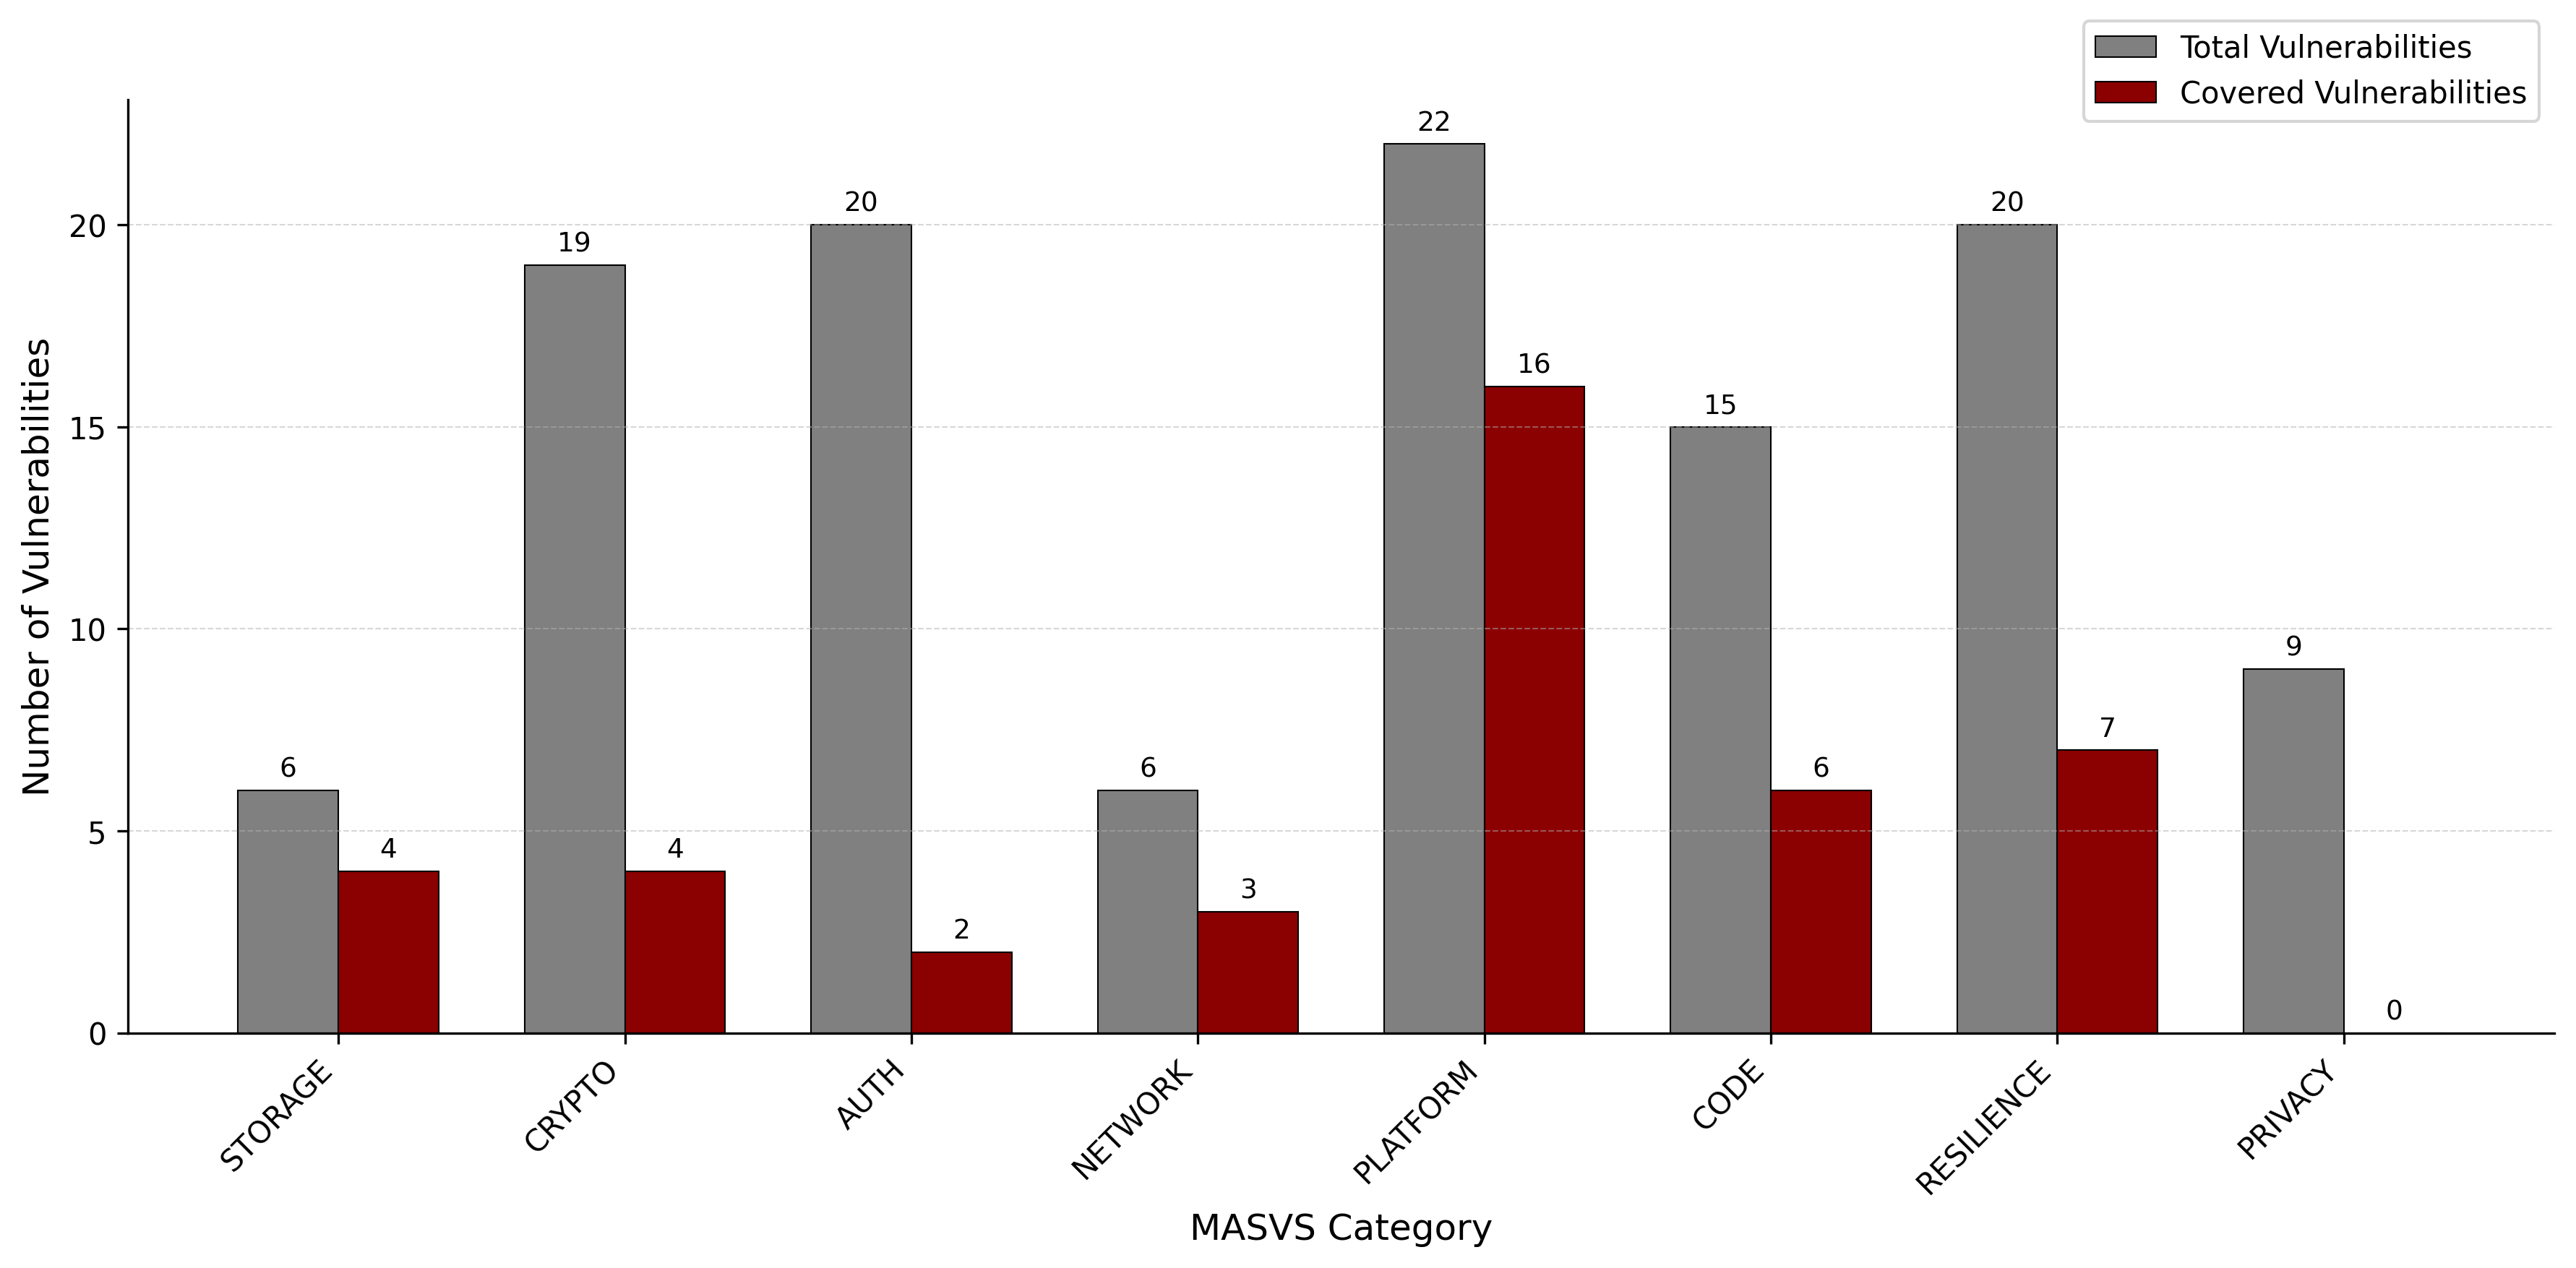
\includegraphics[width=1.0\textwidth]{figures/related_work/vulnerability_coverage_counts.png}
  \caption{Absolute coverage of MASVS categories}
  \label{fig:vulnerability_coverage_absolute_without_own_apps}
\end{figure}

Nevertheless, it can be concluded that the categories are unevenly covered, with MASVS-PLATFORM receiving a great deal more attention than the other categories, and MASVS-PRIVACY receiving none. The coverage of many categories in these MASTG reference apps is lacking, with only 21.1\% and 10\% of all MASVS-CRYPTO and MASVS-AUTH vulnerabilities being covered, respectively. This stands in stark contrast to the amount of material provided on them by the OWASP MAS project. They represent a large part of the mobile security that OWASP deals with, considering they make up a third (39/117) of all vulnerabilities documented by the MASWE and tested for by the MASTG. 

The reference apps we develop aim to solve this issue by focusing on vulnerability types that have not been implemented in existing MASTG reference apps, as well as by shifting the focus from over-represented categories such as MASVS-PLATFORM to more neglected ones, such as MASVS-CRYPTO and MASVS-AUTH.

% Struktur
\section{Literature Review - Academic relevance of OWASP MASTG}
\label{sec:literature_review}
The OWASP MASTG is the industry standard for mobile app security. But what relevance does it have in the academic world, and what exactly is it used for? To answer these questions, a literature review was conducted to evaluate academic publications on their usage of the OWASP MASTG, as well as other parts of the OWASP MAS project.

This literature review was conducted by searching for relevant papers that include and deal with the keywords "OWASP" and "MASTG" on Google Scholar. Only papers written in English were considered. Furthermore, all evaluated papers have been published in the last three years, with no paper having been published prior to 2023. The top 22 papers matching these criteria have been carefully read, with seven of them discarded because their research focus did not match our defined scope. This left 15 papers \citep{paper_01, paper_02, paper_03, paper_04, paper_05, paper_06, paper_07, paper_08, paper_10, paper_13, paper_14, paper_19, paper_20, paper_21, paper_22}, which were then evaluated for their usage of OWASP MASTG and grouped by similarity.

Of the 15 papers evaluated, eight \citep{paper_01, paper_02, paper_03, paper_04, paper_05, paper_07, paper_13, paper_14} used OWASP MASTG to evaluate real-world Android apps based on whether they adhere to the security standard set by OWASP MASVS. Six papers \citep{paper_01, paper_02, paper_03, paper_04, paper_05, paper_07} mapped Android app security vulnerabilities to the OWASP MASVS. Three papers \citep{paper_03, paper_04, paper_06} made use of the penetration testing guide, as laid out by OWASP MASTG, in order to conduct penetration tests on Android apps. Three papers \citep{paper_10, paper_19, paper_22} used the MASTG reference apps by evaluating vulnerability assessment tools on them in order to verify their accuracy in finding such vulnerabilities. Two of these papers \citep{paper_19, paper_22} then compared their findings to results found when conducting the same tests on real-world apps. Lastly, four papers \citep{paper_08, paper_20, paper_21, paper_22} mentioned the OWASP MASTG in discussion. This was done either by the authors, comparing the OWASP mobile project to other Mobile Security Frameworks, or by interviewees, as a tool used. An overview of the different papers and how they made use of the OWASP MAS project can be seen in Table \ref{overview_owasp_mas_usage_academic_world}.

\begin{table}[htpb]
\centering
\caption{Overview of how scientific papers make use of the OWASP MAS project}
\begin{tabular}{ |p{1.2cm}||p{2cm}|p{2cm}|p{2cm}|p{2cm}|p{2cm}|  }
    \hline
    \multicolumn{6}{|c|}{OWASP MAS usage by scientific papers} \\
    \hline
    Paper & Evaluating real-world apps & Vulnerability mapping & Penetration testing guide & Reference apps & In Discussion \\
    \hline
    1 \citep{paper_01}   & \centering\checkmark & \centering\checkmark &   &   &   \\
    \hline
    2 \citep{paper_02}   & \centering\checkmark & \centering\checkmark &   &   &   \\
    \hline
    3 \citep{paper_03}   & \centering\checkmark & \centering\checkmark & \centering\checkmark &   &   \\
    \hline
    4 \citep{paper_04}   & \centering\checkmark & \centering\checkmark & \centering\checkmark &   &   \\
    \hline
    5 \citep{paper_05}   & \centering\checkmark & \centering\checkmark &   &   &   \\
    \hline
    6 \citep{paper_06}   &     &  & \centering\checkmark &   &   \\
    \hline
    7 \citep{paper_07}   & \centering\checkmark & \centering\checkmark &   &   &   \\
    \hline
    8 \citep{paper_08}   &     &  &   &   & \centering\arraybackslash\checkmark \\
    \hline
    9 \citep{paper_10}   &     &  &   & \centering\checkmark &   \\
    \hline
    10 \citep{paper_13}   & \centering\checkmark &  &   &   &   \\
    \hline
    11 \citep{paper_14}   & \centering\checkmark &  &   &   &   \\
    \hline
    12 \citep{paper_19}   &     &  &   & \centering\checkmark &   \\
    \hline
    13 \citep{paper_20}   &     &  &   &   & \centering\arraybackslash\checkmark \\
    \hline
    14 \citep{paper_21}   &     &  &   &   & \centering\arraybackslash\checkmark \\
    \hline
    15 \citep{paper_22}   &     &  &   & \centering\checkmark & \centering\arraybackslash\checkmark \\
    \hline
\end{tabular}
\label{overview_owasp_mas_usage_academic_world}
\end{table}

\subsubsection{Cryptographic security shortcomings in African mobile financial applications}
Chiboora et al. \citep{paper_07} used the OWASP MASTG and the MASVS to evaluate the mobile security of 18 Android apps belonging to different African financial institutions. They chose MASVS as a testing framework because of its focus on being a guide and checklist for evaluating the security of mobile applications. They applied the strictest level of MASVS, L2, and focused solely on unauthenticated client-side testing, following the black-box testing approach. They did not implement all MASVS tests. Nevertheless, their findings in terms of security shortcomings are quite damning. All 18 apps allowed the taking of screenshots of sensitive data. 14 of the apps used outdated and thus insecure cryptographic protocols such as MD5, SHA-1, and DES. 10 apps used security libraries that are outdated and known to have vulnerabilities. Furthermore, eight apps were using insecure random number generation for their cryptographic protocols, and five apps had no certificate pinning. This shows a clear and dramatic shortcoming in terms of cryptographic mobile security. All of the shortcomings mentioned above are well documented by the OWASP MASWE, tested for by the MASTG, and are part of the security controls of the MASVS. This shows that the OWASP MAS project has a great use case in the real world, and is far from being outdated or redundant. In a survey conducted by the authors of this study, 78\% of respondents said they avoided implementing security measures due to a lack of expertise and knowledge about mobile security. We aim to increase the coverage of MASVS-CRYPTO vulnerabilities through our intentionally vulnerable reference apps. This addresses an important shortcoming in the current landscape of available MASTG reference apps, which do not cover the MASVS-CRYPTO category sufficiently. This decision concurs with the issues found and discussed in this paper by enabling mobile developers to deepen their expertise and knowledge of cryptographic vulnerabilities in a hands-on way.

\subsubsection{Lack of basis for Mutation Testing for Android app security testing}
Vasconcelos et al. \citep{paper_10} explored Mutation Testing as an approach for Android app security testing. The authors used the OWASP Top 10 Mobile Risks to assess common Android security vulnerabilities and created mutation operators based on these vulnerabilities. They then performed security tests on the mutants generated by the mutation operators, in the hope that these mutants would be detected as vulnerabilities. They applied this procedure to 10 Android reference apps from the MASTG reference app catalog. They found that four of the eight generated mutant operators were not represented among the mutants at all, while two other were heavily overrepresented. To be more specific, all three tapjacking vulnerability mutant operators and the "ImplicitPendingIntent" operator have no representation in the apps, whereas "ImproperExport" and "HardcodedSecret" are both heavily overrepresented. This corroborates our own findings upon analyzing the implemented vulnerabilities in the reference apps. Only one of the 163 vulnerabilities implemented by the MASTG reference apps deals with tapjacking attacks. The same applies to implicit pending intents. On the contrary, eight vulnerabilities deal with hard-coded secrets. Because of uneven distribution of implemented vulnerabilities, some mutants are generated more frequently than others. This shows that the large number of MASWE vulnerability types that go without a practical implementation in the reference apps affects the academic world as well. By focusing on these vulnerabilities for the development of our reference apps, we aim to address this issue. 

\subsubsection{Security shortcomings in the American mHealth sector}
Stevenson and Das \citep{paper_14} used the OWASP Mobile Audit to evaluate 95 real-world apps that are part of the mobile health sector in the USA. The OWASP Mobile Audit is an OWASP project that applies SAST aligned with the MASTG to detect mobile security vulnerabilities. The findings were quite devastating. These apps dealing with sensitive user health data had, on average, around 9,000 vulnerabilities, with two thirds of them being of medium to critical severity. Around half of the evaluated apps transmit data containing personal health information with no encryption over HTTP, or make use of heavily outdated cryptographic algorithms. Furthermore, they found 2,252 instances of unnecessarily exported broadcast receivers and 1,232 cases of exported permissions without defined protection levels. 

This paper underlines the significant shortcomings of apps in the cryptographic sector of mobile security, even when it comes to sensitive user data. All of the found vulnerabilities are well documented by the MASWE, and would not exist anymore if developers followed the standards laid out by the OWASP MAS project. The authors conclude that the overall lack of security measures implemented is further worsened by the fact that the developers follow insecure coding practices. The authors specifically recommend the OWASP MASVS as the security standard that mobile developers should adopt. This paper emphasizes the real-world importance of the OWASP MASVS, the MASTG, and the related reference apps. Many of the vulnerabilities detected by the OWASP Mobile Audit deal with cryptographic issues, which is a MASVS category with very limited coverage by existing MASTG reference apps. The reference apps we develop aim to address this issue by focusing on vulnerabilities documented in MASVS-CRYPTO.

\subsubsection{Security Assessment for Digital Wallet Payment Partner Applications using the OWASP Method: A Case Study in Indonesia}
Saifulhakim and Fajar \citep{paper_02} made use of the OWASP MASTG and MASVS to assess the security standards of a digital wallet payment partner mobile app. The authors applied both dynamic (DAST) and static (SAST) application security testing. They mapped the found vulnerabilities to the MASWE and used the OWASP Risk Rating Methodology to assess the security risks of the detected vulnerabilities. They identified vulnerabilities using both the static and dynamic approach.  The paper found that of the 84 MASVS verification points, 68 were met, 10 were deemed not applicable, and six failed due to vulnerabilities found. The authors referenced multiple papers and articles demonstrating that the OWASP MAS project presents a viable solution for security assessment. They note that financial transaction apps are particularly common to have a high vulnerability rate, and that insecure data storage occurs more frequently than other vulnerabilities types. 

This paper shows that MASTG reference apps should include both dynamic and static vulnerabilities if they desire to mimic real-world app vulnerabilities. It goes on to discuss the high frequency in which storage vulnerabilities occur. The reference apps we develop build on these findings by including both static and dynamic vulnerabilities. Our reference apps aim to implement MASWE vulnerabilities related to storage. By doing so, our apps reflect vulnerabilities as they are found in real-world apps.

\subsubsection{SoK: Hardening Techniques in the Mobile Ecosystem — Are We There Yet?}
The OWASP MASVS advises mobile app developers to implement so called hardening techniques. They serve as a layer of device protection by preventing tampering with the device and detecting jailbreaks. Steinböck et al. \citep{paper_22} investigated the extent to which real-world apps adhere to the MASVS and implement such hardening techniques. To do so, they created HALY, a framework that allows for static as well as dynamic analysis of the adoption of hardening techniques in mobile apps. They discuss how MASVS-RESILIENCE specifies multiple hardening techniques that apps should implement as to conform to modern security standards. They used the MASVS as a base of operations since the MASVS is the standard used for Android apps that opt into Google Play’s independent security review process \citep{paper_22}. This shows the importance of the recommendations and practices laid out in the standards established by the OWASP MAS project. Their framework HALY is built to detect vulnerabilities in three of the four categories defined by MASVS-RESILIENCE. The authors validated the accuracy of their framework by testing it on seven open source apps, including four Android and two iOS OWASP reference apps. They proceeded to use their framework to evaluate 2,646 apps, both available on Android and iOS, for their use of hardening techniques. Their findings show that iOS apps heavily under-perform when it comes to implementing hardening techniques, as opposed to apps on Android devices. Of the 2,646 apps evaluated, about 75\% of Android and 25\% of iOS apps implement more than half of the protection techniques recommended by MASVS-RESILIENCE. Only 26 Android apps adopt all eight, while only one iOS app adopts all seven. This paper shows the real-world importance of the MASVS through its role as the standard used in Google Play's data safety section. It displays the merit of the MASTG reference apps and the MASVS to the academic world as a basis on which to conduct important research. Their findings show that there are still many mobile apps that do not follow the security best practices defined by OWASP. The MASTG reference apps we develop provide a basis on which future academic work similar to this paper can build on. They furthermore serve as an example from which mobile developers can learn to improve the security standards of mobile apps used globally.